% ARROW manuscript, provisionally using the official CVPR 2026 author kit.
\documentclass[10pt,twocolumn,letterpaper]{article}
\usepackage[review]{cvpr}
% ARROW paper preamble. Keep dependencies available in a standard TeX Live.
\usepackage{amsmath,amssymb}
\usepackage{booktabs}
\usepackage{graphicx}
\usepackage{multirow}
\usepackage{xcolor}
\usepackage{xspace}
\usepackage{microtype}
\usepackage{enumitem}
\usepackage{placeins}

\newcommand{\method}{\textsc{Arrow}\xspace}
\newcommand{\arrowv}{\textsc{Arrow-V}\xspace}
\newcommand{\arrowt}{\textsc{Arrow-T}\xspace}
\newcommand{\arrown}{\textsc{Arrow-N}\xspace}
\newcommand{\sg}{\operatorname{sg}}
\DeclareMathOperator*{\argmaxop}{arg\,max}

% Generated by paper/scripts/make_main_tables.py.
\newcommand{\ArrowTestGain}{+2.08}
\newcommand{\ArrowTestGainLo}{1.83}
\newcommand{\ArrowTestGainHi}{2.35}
\newcommand{\ArrowStrictGain}{4.19}
\newcommand{\ArrowStrictGainLo}{2.46}
\newcommand{\ArrowStrictGainHi}{6.20}
\newcommand{\ArrowOwnershipStrictGain}{2.81}
\newcommand{\ArrowVisualSwitch}{48.2}
\newcommand{\ArrowTextSwitch}{32.3}
\newcommand{\ArrowNullSwitch}{0.0}
\newcommand{\ArrowFineCopsCoverage}{95.60}
\newcommand{\ArrowFineCopsFixedTPR}{80.05}
\newcommand{\ArrowGrefFixedTPR}{90.10}



\definecolor{cvprblue}{rgb}{0.21,0.49,0.74}
\usepackage[pagebackref,breaklinks,colorlinks,allcolors=cvprblue]{hyperref}

\def\paperID{*****}
\def\confName{CVPR}
\def\confYear{2027}

\title{ARROW: Factorizing Admission, Ranking, and Abstention\\for Selective Visual Grounding}
\author{Anonymous CVPR submission}

\begin{document}
\maketitle

\begin{abstract}
Selective grounding must decide which candidates may compete, which candidate
wins, and whether any winner should be emitted.  \method factorizes these as
\emph{Admission}, \emph{Ranking}, and \emph{Abstention} over frozen grounding
queries.  Its released ARROW-U2 instance improves a five-split RefCOCO-family
endpoint by 2.08 points and reduces verified-negative FPR95 by 4.19 points,
without letting confidence alter the selected box.  Capacity-matched controls
show that Ranking--Abstention interference depends on representation strength:
isolation recovers 5.31 localization points on one frozen representation, but
broad pretrained and RefCOCO-tuned MM-GDINO representations support wide
sharing, even when TN exposure deepens the negative-gradient tail.  A
fresh category-switch test distinguishes learned-null, category-text, and
visual-support Admission despite similar standard accuracy.  FineCops-Ref and
restricted gRefCOCO further show that rejection ordering transfers more
reliably than a fixed operating threshold.  Thus ARROW supports decision
factorization and measured, rather than universal, owner isolation.
\end{abstract}

\section{Introduction}
\label{sec:intro}

Referring-expression comprehension usually assumes that every expression
denotes exactly one object in the image.  A deployed system cannot rely on
this assumption: a request may be invalid, stale, or unsupported by the
current scene, and the system must decide whether to localize or abstain.
Generalized referring-expression benchmarks make absence explicit by
including no-target cases~\cite{ding2026grex}.  The practical problem is
therefore not only to predict a box, but to emit a box \emph{selectively}.

Detector-style grounding models expose text-conditioned queries and matching
scores~\cite{liu2025groundingdino}.  In practice, a score is often asked to do
three jobs: filter category-ineligible candidates, order the remaining
instances by the complete expression, and determine whether any candidate
should be accepted.  These jobs have different semantics.  \emph{Admission}
constructs a comparison set, \emph{Ranking} is relative within that set, and
\emph{Rejection} is a sample-level decision.  A ranker must always choose a
winner, even when every candidate is invalid; a rejector must instead suppress
the entire sample.  Coupling these decisions is consequently an optimization
problem rather than a naming inconvenience, as the cases in
Fig.~\ref{fig:teaser} illustrate.

We begin from a frozen, data-finetuned Grounding DINO representation.  Across
26,488 validation expressions per seed, its all-query geometry contains an
IoU$\geq0.5$ candidate in every case.  Admission removes the final compatible
candidate in only 0.31--0.38\% of examples, yet 27.23--27.39\% remain ranking
errors inside the eligible set.  A shared-scalar Admission/Rejection control
exposes a second failure: the two gradients have negative mean cosine in all
three seeds.  Separate outputs over the same trainable feature owner barely
change calibration FPR95, whereas disjoint owners improve rejection without
changing the localization route.

We therefore introduce \method: \textbf{Admission, Ranking, and Rejection with
Ownership-Separated Weights}.  A frozen generator supplies candidates.
Admission uses an optional category cue to construct an eligible set.  The
complete expression ranks candidates within that set.  An independent
sample-level score then accepts or rejects the result.  Every deployed surface
has an exclusive trainable owner.  A dashed auxiliary route can carry
Admission supervision during training, but it never enters a deployed decision
score and cannot become a hidden fourth score.  \arrowv uses a visual support exemplar;
\arrowt uses an explicit canonical category phrase without a visual support
image; \arrown is a category-agnostic mechanism control.  The category cue is
separate from the complete expression that still owns geometry and Ranking.

\begin{figure*}[t]
  \centering
  \IfFileExists{figures/fig1_teaser.pdf}{%
    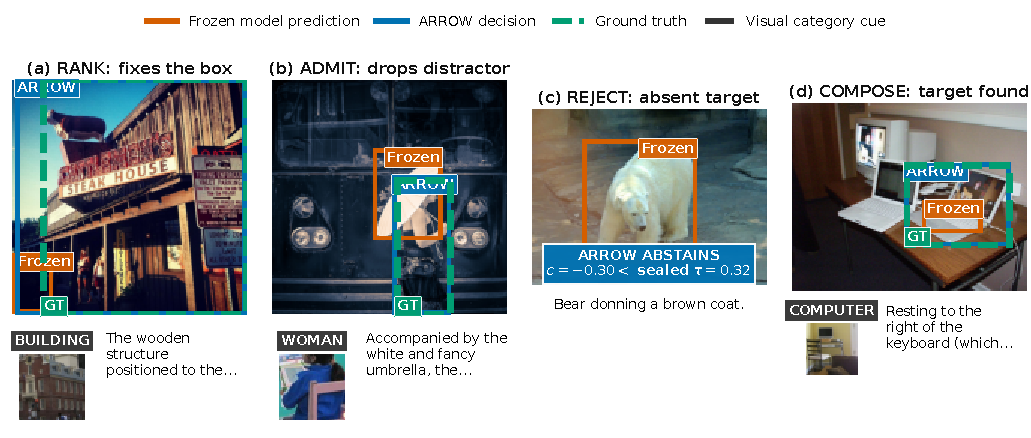
\includegraphics[width=\textwidth]{figures/fig1_teaser.pdf}%
  }{\fbox{\parbox[c][1.15in][c]{0.96\textwidth}{\centering
    Deterministically selected candidate, Admission, and no-target examples
    will be generated from sealed records.}}}
  \caption{A valid candidate may already exist; reliable grounding must learn
  who enters, who wins, and whether any winner should be emitted, without
  allowing the three duties to overwrite one another.  Zero-training examples
  are selected from sealed records by deterministic predicates; panel (d)
  adds a level-3 compositional success.  Failure cases remain in the
  qualitative supplement.  Detached cue tiles
  below panels (a), (b), and (d) are external Admission inputs, not crops from
  the evaluated detection image.}
  \label{fig:teaser}
\end{figure*}

Our evidence supports three claims.  First, the factorized route improves the
frozen base on both held-out localization and verified rejection.  Second,
exclusive ownership---not output count alone---removes the measured conflict.
Third, ordinary endpoint accuracy hides functional responsibility: \arrown
retains much standard accuracy but cannot switch category; text provides
explicit control, and visual support adds evidence beyond the name alone.
FineCops-Ref~\cite{liu2024finecops} gives a descriptive discrimination gain,
and paired results on a restricted single/no-target gRefCOCO slice confirm it.
The sealed threshold misses 95\% TPR on both external surfaces.

Our contributions are:
\begin{enumerate}[leftmargin=*,itemsep=1pt,topsep=2pt]
  \item \textbf{Deployment-duty factorization.} We formulate single-target
  selective grounding as Admission, Ranking, and Rejection, and diagnose
  failures after adequate candidate geometry already exists.
  \item \textbf{Responsibility-isolated optimization.} Controlled comparisons
  show that separate outputs sharing a trainable feature owner are
  insufficient, whereas structural cross-duty isolation preserves
  localization and improves rejection.
  \item \textbf{Functional and external validation.} Category-switch
  interventions distinguish generic, textual, and visual Admission, while two
  external negatives give descriptive FineCops evidence and paired gRefCOCO
  confirmation while exposing fixed-threshold shift.
\end{enumerate}

\section{Related Work}
\label{sec:related}

\paragraph{Text and visual prompts.}
Open-vocabulary grounding and detection models such as Grounding
DINO~\cite{liu2025groundingdino} use language to define detection concepts.
T-Rex2~\cite{jiang2024trex2} aligns text and visual prompts, while PET-DINO
adds visual cues and parallel prompt routes to Grounding
DINO~\cite{fu2026petdino}.  DINO-X broadens the available prompt types, and
Visual In-Context Prompting introduces the DINOv visual-prompt
model~\cite{ren2024dinox,li2024dinov}.  \method does not claim novelty in
accepting both modalities.  Its question is decision-level responsibility: a
category cue controls Admission, while the complete referring expression owns
within-set Ranking.  The fresh category-switch intervention tests whether each
route actually follows its assigned cue.

\paragraph{Referring expressions and no-target grounding.}
RefCOCO and RefCOCO+~\cite{yu2016modelingcontext} and
RefCOCOg~\cite{mao2016generation} support the classical exactly-one-target
setting.  gRefCOCO was introduced with the generalized segmentation task
GRES~\cite{liu2023gres}; the subsequent GREC formulation applies it to
zero-, one-, and multiple-target comprehension~\cite{he2023grec}, and the
peer-reviewed GREx account unifies the benchmark lineage across segmentation,
comprehension, and generation~\cite{ding2026grex}.  RECANTFormer directly
predicts varying-size target sets with an encoder-only Transformer and
Hungarian matching~\cite{hemanthage2024recantformer}; HieA2G instead estimates
target cardinality with an adaptive counter~\cite{wang2025hiea2g}.  Related
instance-aware methods align phrases to instances or jointly predict boxes and
masks~\cite{nguyen2024instalign,dai2026instancevg}, while RC-GRPO balances
localization and refusal in an MLLM policy~\cite{yang2026rcgrpo}.
FineCops-Ref~\cite{liu2024finecops} probes fine-grained positive grounding and
counterfactual negative expressions/images.  We do not claim the first
no-target head or full variable-cardinality grounding.  Instead, we isolate a
narrower question in a specialist detector: which parameters may own each
deployed decision?  Our gRefCOCO experiment is explicitly restricted to
single-target versus no-target expressions.

\paragraph{Multi-task interference and parameter isolation.}
Gradient methods such as GradNorm~\cite{chen2018gradnorm},
PCGrad~\cite{yu2020pcgrad}, and CAGrad~\cite{liu2021cagrad} rebalance or
modify gradients on shared parameters.  Adapters and LoRA allocate lightweight
task-specific capacity~\cite{houlsby2019adapters,hu2022lora}.  \method is not a
general gradient-surgery rule.  The deployment policy defines ownership: a
loss may update only the owner of the surface that executes that duty.  This
produces structural zero cross-duty gradients rather than a numerical
correction to a shared gradient.  Freezing the candidate representation also
preserves geometry shown empirically to be sufficient for the analyzed data.

\section{Problem Formulation and Diagnosis}
\label{sec:problem}

\subsection{Selective single-target grounding}
Given an image $I$, complete referring expression $e$, and optional category
cue $u$, the deployed policy returns one box or abstention:
\begin{equation}
  \hat y=\pi(I,e,u)\in\mathcal{B}\cup\{\varnothing\}.
\end{equation}
A frozen grounding model produces $N$ candidate queries,
\begin{equation}
  \mathcal{Q}=G_{\phi}(I,e)
  =\{(q_i,b_i,s_i^0)\}_{i=1}^{N},\qquad \phi\ \text{frozen}.
\end{equation}
The policy must decide which candidates may compete, which admitted candidate
best satisfies $e$, and whether the selected result is sufficiently supported
to emit.

\subsection{Three different decision semantics}
Admission constructs an eligible set $\mathcal{E}\subseteq\{1,\ldots,N\}$.
Ranking is relative:
\begin{equation}
  i^*=\argmaxop_{i\in\mathcal{E}} r_i(I,e).
\end{equation}
A maximum exists even on a no-target sample.  Abstention is sample-level:
\begin{equation}
  \hat y =
  \begin{cases}
    b_{i^*}, & c(I,e)\geq\tau,\\
    \varnothing, & c(I,e)<\tau.
  \end{cases}
\end{equation}
It should separate samples with a valid referent from invalid pairs without
changing within-set order.  A shared trainable owner may support both
objectives, or the updates may interfere.  For a shared owner $\Theta_S$, we
measure
\begin{equation}
  \kappa =
  \cos\!\left(\nabla_{\Theta_S}\mathcal{L}_{R},
              \nabla_{\Theta_S}\mathcal{L}_{C}\right)
\end{equation}
and test endpoint behavior under capacity-matched sharing and isolation.  The
sign and consequence of $\kappa$ depend on the representation, owner capacity,
data, and optimization state; they do not follow from the task names alone.

\subsection{Candidate-availability diagnosis}
We partition localization outcomes into four cases: no IoU$\geq0.5$ candidate
exists; Admission removes the last compatible candidate; a valid admitted
candidate exists but Ranking selects another; or localization is correct but
Abstention falls below the operating threshold.  On the analyzed frozen-base
validation surface, the first class is empty, the second accounts for only
0.31--0.38\%, and 27.23--27.39\% remain Ranking errors.  This diagnoses one
representation and evaluation surface; it does not claim that candidate
geometry is universally solved.

\section{ARROW}
\label{sec:method}

\begin{figure*}[t]
  \centering
  \IfFileExists{figures/fig2_method_ownership.pdf}{%
    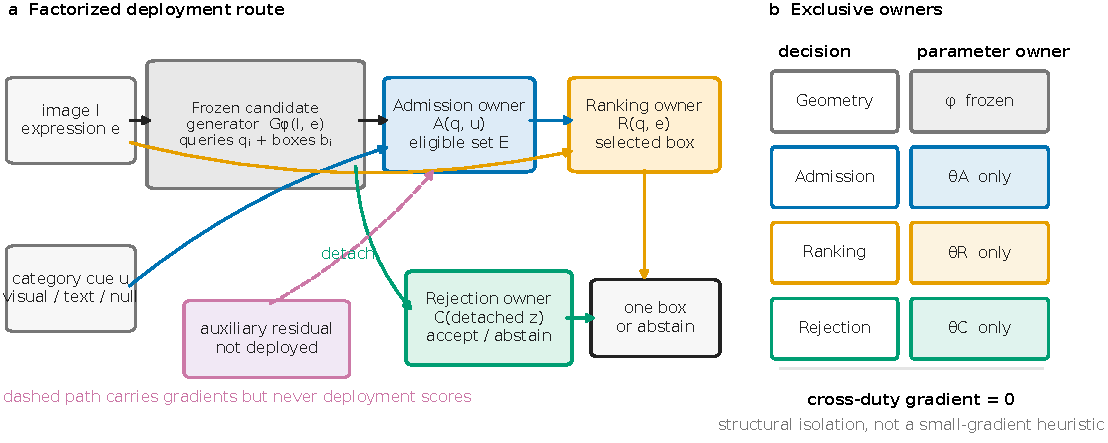
\includegraphics[width=\textwidth]{figures/fig2_method_ownership.pdf}%
  }{\fbox{\parbox[c][1.35in][c]{0.96\textwidth}{\centering
    Frozen candidates $\rightarrow$ Admission $\rightarrow$ Ranking; detached
    evidence $\rightarrow$ Abstention.}}}
  \caption{\method factorizes the deployed policy without prescribing one
  universal parameter topology.  Admission defines the comparison set,
  Ranking selects within it, and Abstention decides whether the selected box is
  emitted.  ARROW-U2 isolates Ranking and Abstention; matched controls test
  shared and isolated owner allocations.  The auxiliary Admission residual is
  serialized and computed for compatibility but ignored by every deployed
  decision score.}
  \label{fig:method}
\end{figure*}

\subsection{Frozen full-expression candidates}
\method retains the full-expression Grounding DINO candidate generator.  The
complete expression always enters the language encoder, transformer, decoder,
and box predictor; neither a canonical noun nor a generic ``object'' prompt
replaces this geometry path.  The frozen generator returns boxes $b_i$,
final-decoder queries $h_i$, and native scores $s_i^0$.  Freezing keeps
candidate geometry and base evidence identical across cue and owner controls.

\subsection{Category-conditioned Admission}
Let $u$ denote the category cue.  Admission computes
$\bar u=P_{\theta_A}(u)$ and
\begin{equation}
  a_i=\alpha\cos(W_{\theta_A}h_i,\bar u).
\end{equation}
Scores are standardized inside the valid-candidate mask $\mathcal{M}$,
yielding $\tilde a_i$.  The deployed relative-margin gate is
\begin{equation}
  \mathcal{E}_{\gamma}
  =\{i\in\mathcal{M}:
  \max_{j\in\mathcal{M}}\tilde a_j-\tilde a_i\leq\gamma\},
  \qquad \gamma=3.
  \label{eq:admission}
\end{equation}
The maximum-score valid query is necessarily admitted.  Missing valid
candidates, non-finite scores, or an empty set fail closed.  Eligible rank
scores remain bitwise equal to the frozen ranker; ineligible queries are
lexicographically demoted, so Admission changes membership but not within-set
order.

We instantiate three capacity-matched cues.  Visual-support Admission encodes
an external exemplar with a frozen patch backbone.  Category-text Admission
encodes a canonical category phrase with the frozen language encoder without
rerunning image decoding.  Learned-null Admission uses a fixed
category-agnostic sentinel transformed by the same trainable surface.  All
three use the same candidate mask, gate, losses, and Admission capacity.

\paragraph{Supervision-only carrier.}
A small MLP predicts an auxiliary residual $\delta_i^A$ from standardized
Admission and Ranking statistics and forms
$r_i^{\mathrm{aux}}=r_i+\delta_i^A$.  Its losses provide category-complete,
repair, preserve, and regularization supervision.  The implementation retains
this output for checkpoint compatibility, but neither $\delta_i^A$ nor
$r_i^{\mathrm{aux}}$ enters Eq.~\eqref{eq:admission}, deployed Ranking, or the
final emit/abstain decision.

\subsection{Complete-expression Ranking}
Within the eligible set, the positive-only ranker uses the complete expression:
\begin{equation}
  r_i=R_{\theta_R}(q_i,e),\qquad
  i^*=\argmaxop_{i\in\mathcal{E}_{\gamma}} r_i .
\end{equation}
It learns a bounded residual over the frozen full-expression score.  Training
repairs a wrong base top-1 while preserving an already-correct
positive--negative gap, and Ranking is frozen before final Admission and
Abstention training.  Replacing only the Ranking expression by the canonical
noun, while holding geometry and eligibility fixed, changes 37.85\% of top-1
queries and reduces validation Acc@0.5 from 72.46\% to 61.72\%.

\subsection{Sample-level Abstention}
For each query, let $s_i$ be the mean of sigmoid-transformed logits over the
complete expression.  From detached $[h_i,s_i]$, the Abstention module forms a
pooled query feature and concatenates six detached score statistics: maximum,
top-3 mean, mean, standard deviation, top-1--top-2 margin, and normalized
pooling entropy.  An MLP returns one image--expression offset $g$, giving
\begin{equation}
  c(I,e)=\max_i(s_i+g)=\max_i s_i+g.
\end{equation}
Admission and Ranking scores are not inputs.  Deployment emits $b_{i^*}$ when
$c\geq\tau$ and abstains otherwise.  We call $c$ sample-level or non-relative:
``absolute'' distinguishes it from candidate ordering and does not imply a
universally calibrated probability.  The source threshold $\tau$ is sealed
before external evaluation.

\subsection{Responsibility allocation}
The factorized surfaces are logically distinct even when an implementation
shares internal adaptation parameters.  We therefore separate what decision a
surface executes from how its trainable representation is allocated.

ARROW-U2 uses disjoint Ranking and Abstention owners,
\begin{equation}
  \Theta_R\cap\Theta_C=\varnothing,\qquad
  \nabla_{\Theta_R}\mathcal{L}_C=
  \nabla_{\Theta_C}\mathcal{L}_R=0,
\end{equation}
and stop-gradient prevents Abstention from changing candidate geometry or the
selected localization route.  This is a structural guarantee of that
instantiation, not the general definition of \method.  Capacity controls also
train a narrow shared owner, a wide shared owner matched to the isolated
parameter/MAC budget, and two isolated owners.  These controls test whether a
given frozen representation supports soft internal specialization or requires
hard separation.

\section{Experiments}
\label{sec:experiments}

\subsection{Research questions}
We ask whether factorization improves localization and rejection (RQ1),
whether separate heads suffice without exclusive ownership (RQ2), what
information generic/textual/visual Admission carries (RQ3), whether rejection
ordering transfers across independently constructed negative distributions
(RQ4), and whether the source operating threshold transfers unchanged (RQ5).

\subsection{Internal localization and rejection}
Our primary localization endpoint, \textbf{Test5}, is the micro-averaged
Acc@0.5 over RefCOCO testA/testB, RefCOCO+ testA/testB, and RefCOCOg UMD test.
It contains 30,969 expressions from 3,982 images.  Validation splits used for
checkpoint selection are not included.  Ref8, which includes those validation
splits, is descriptive only.

\textbf{Strict-TN2031} contains 2,031 positive/edited-negative pairs on 1,045
images.  Negatives are proposal-covered and verified by a SAM3+VLM pipeline;
they are neither image-global nor all-query verified.  The rejection owner
uses a 14,196-row training surface and a separately sealed 1,570-row
calibration surface; their image sets are mutually disjoint and both are
image-disjoint from Strict-TN2031.  FPR95 sets the threshold
at the positive q05 and measures the negative false-positive rate.  The nested
1,607-pair surface is derived from the same forward and is not treated as an
independent replication.

\subsection{Admission interventions}
The standard Ref evaluation compares \arrowv, \arrowt, and \arrown on identical
frozen geometry/ranking/rejection routes.  A separate fresh panel contains 512
LVIS~\cite{gupta2019lvis} image pairs (1,024 active-category arms) and is image-disjoint from
Admission training, Ref8, and Strict-TN2031.  Its primary metric requires both
directions of a category intervention to score an IoU$\geq0.5$ query for the
active category above the counterfactual category; missing either category's
oracle query counts as failure.

\subsection{External benchmarks}
\paragraph{FineCops-Ref.}
We evaluate all 9,605 positives, 9,814 negative expressions, and 8,507 negative
images using the official byte-exact GQA imagery and pinned evaluator.  No
FineCops train/validation data, checkpoint choice, Admission margin, support
alias, or threshold fit is used.  \arrowv has an exact preregistered support
mapping for 9,182 positives (\ArrowFineCopsCoverage\%); its matched contrasts
include only pairs for which both arms are supported.  The full-test \arrowt
route receives the benchmark's structured target noun as its explicit
canonical cue.  Published detector numbers are therefore a numerical reference,
not an input-matched controlled comparison.  This is
FineCops-specific annotation/task zero-shot, not a claim of global image
disjointness.

\paragraph{gRefCOCO.}
We evaluate a restricted binary slice: 11,563 single-target expressions are
positive and 9,121 no-target expressions are negative; all 14,579 multi-target
expressions are excluded.  This is not full 0-to-$N$ GREC.  All 1,500 images
were exposed during Stage-A.  The paper-facing
\emph{Rejector-supervision-disjoint} subset removes the 182 images used for
rejector training and 30 used for rejector calibration, retaining 1,288
images, 9,924 positives, and 7,796 no-target negatives.  It is not globally
image-disjoint.

\subsection{Metrics and statistical protocol}
Localization uses Acc@0.5 or benchmark P@1.  Rejection uses AUROC, positive
AUPR, and FPR95.  External fixed-threshold results apply each seed's sealed
source threshold without modification.  We report per-seed values, their mean,
and sample SD.  Confirmatory intervals use 5,000 paired image-cluster (or
parent-image-cluster) bootstrap replicates with PCG64.  The same cluster draw
is applied to both models and all seeds.  Every FPR95 replicate recomputes each
model's q05 from that replicate's positive clusters; the fixed deployment
threshold is never recomputed.  Planned families use Holm correction.

\subsection{Implementation and frozen decisions}
The candidate generator, visual backbone, language encoder, decoder, and
positive-only complete-expression ranker remain frozen during final Admission
and Rejection training.  Admission and Rejection are trained in separate
phases with disjoint optimizer ownership.  All formal routes use three seeds
(17, 42, 73), fixed update counts, a relative Admission margin $\gamma=3$, and
the preregistered checkpoint-selection rule.  No model, margin, queue, or
threshold is changed after a held-out or external result.  Exact parameter,
latency, and memory measurements follow the no-training efficiency protocol in
the supplementary material.

\section{Results}
\label{sec:results}

% Generated by paper/scripts/make_main_tables.py.
\begin{table*}[t]
\centering
\caption{Held-out system endpoints.  Admission and Ranking determine the
localization route; adding Abstention leaves every selected query and box
bitwise unchanged.  Deltas and paired 95\% image-cluster intervals are relative
to the frozen base.}
\label{tab:headline}
\scriptsize
\setlength{\tabcolsep}{3.1pt}
\begin{tabular}{lrrrrrr}
\toprule
System & Test5$\uparrow$ & Strict FPR95$\downarrow$ & $\Delta$Test5 [CI] & FPR95 red. [CI] & Elig. recall$\uparrow$ & Elig. $n\downarrow$ \\
\midrule
Frozen base & 72.16 & 51.21 & -- & -- & -- & -- \\
Admission + Ranking & 74.24 & -- & +2.08 [1.83, 2.35] & -- & 99.69 & 69.5 \\
ARROW-U2 (+ Abstention) & 74.24 & 47.02 & +2.08 [1.83, 2.35] & 4.19 [2.46, 6.20] & 99.69 & 69.5 \\
\bottomrule
\end{tabular}
\vspace{2pt}
\parbox{0.98\textwidth}{\footnotesize Percentages except eligible-query
count.  Frozen-to-ARROW rows are cumulative system comparisons with additional
head supervision; equal-supervision owner claims use
Tab.~\ref{tab:interference}.  Validation decomposition and parameter/runtime
accounting are supplementary.}
\end{table*}


\subsection{ARROW improves both deployed endpoints}
\method improves Test5 Acc@0.5 by \ArrowTestGain\ points (95\% paired
image-cluster CI [\ArrowTestGainLo, \ArrowTestGainHi]) and lowers
Strict-TN2031 FPR95 by \ArrowStrictGain\ points (CI
[\ArrowStrictGainLo, \ArrowStrictGainHi]); see Tab.~\ref{tab:main}.
Rejection cannot explain the localization gain: learned Admission plus Ranking
and full \arrowv have bitwise-identical localization records by construction.

The cumulative mechanism rows explain complementarity rather than independent
additivity.  The unrestricted complete-expression ranker is almost identical
to the base.  A static Admission prior helps modestly, and learned Admission
creates the main localization gain by constraining the comparison domain.  Yet
canonicalizing only the ranking expression---with geometry and eligibility
fixed---drops Acc@0.5 by more than ten points and changes 37.85\% of top-1
queries.  Admission defines who may compete; the complete expression decides
which instance wins.

% Generated by paper/scripts/make_main_tables.py.
\begin{table*}[t]
\centering
\caption{Ownership evidence at two representation strengths.  On ARROW-U2,
isolation improves rejection with unchanged localization.  On the strong e5
trunk, Isolated reduces FPR95 by 4.070 points versus Native without
changing REC, but does not beat capacity-matched Shared-Wide.}
\label{tab:ownership}
\scriptsize
\setlength{\tabcolsep}{3.5pt}
\begin{tabular}{llrrrrr}
\toprule
Trunk & Design & Params (K) & MAC/query (K) & Grad. cosine (three seeds) & REC$\uparrow$ & Strict FPR95$\downarrow$ \\
\midrule
ARROW-U2 & Shared scalar & -- & -- & -0.19/-0.25/-0.28 & 74.30 & 50.11 \\
ARROW-U2 & Isolated & -- & -- & zero & 74.30 & 47.30 \\
Strong e5 & Native e5 & 0 & 0.0 & -- & 88.969 & 88.282 \\
Strong e5 & Shared-128 & 50.3 & 49.5 & -0.063/+0.008/-0.011 & 88.973 & 85.442 \\
Strong e5 & Shared-Wide & 100.4 & 99.4 & -0.018/+0.032/+0.012 & 88.979 & 83.686 \\
Strong e5 & Isolated & 100.4 & 98.8 & zero by design & 88.976 & 84.211 \\
\bottomrule
\end{tabular}
\vspace{2pt}
\parbox{0.98\textwidth}{\footnotesize ARROW-U2 REC is Test5; strong-e5 REC
is RefCOCO TestA+TestB micro. Learned rows report three-seed means; Native is
deterministic. Shared-Wide and Isolated match total capacity
(100,362 vs. 100,358 parameters); Shared-Wide also gives each task a wider
210-d representation. Separate task-specific Adam states and zero weight decay
are used in every learned arm. The e5 trunk is a retrospective checkpoint
replay; its ownership matrix was frozen prospectively.}
\end{table*}


\subsection{Ownership, not output count, resolves conflict}
Table~\ref{tab:ownership} isolates feature ownership from output separation.
The shared scalar has negative Admission/Rejection gradient cosine in every
seed ($-0.190$, $-0.252$, $-0.281$), with sign-conflict fractions around
0.53--0.56.  Merely attaching separate outputs to the same trainable feature
surface leaves calibration FPR95 essentially unchanged; this separate-head
control is calibration-only and has no held-out Strict result.  Removing the
shared autograd path lowers it substantially.  On held-out endpoints, isolated owners
change Test5 by only $-0.002$ points while reducing Strict-TN2031 FPR95 by
\ArrowOwnershipStrictGain\ points.  Phased exposure is non-inferior in
localization but has no significant rejection improvement over already
isolated interleaving; our claim is structural ownership isolation, not a
schedule advantage.

\begin{figure*}[t]
  \centering
  \IfFileExists{figures/fig3_mechanism_controllability.pdf}{%
    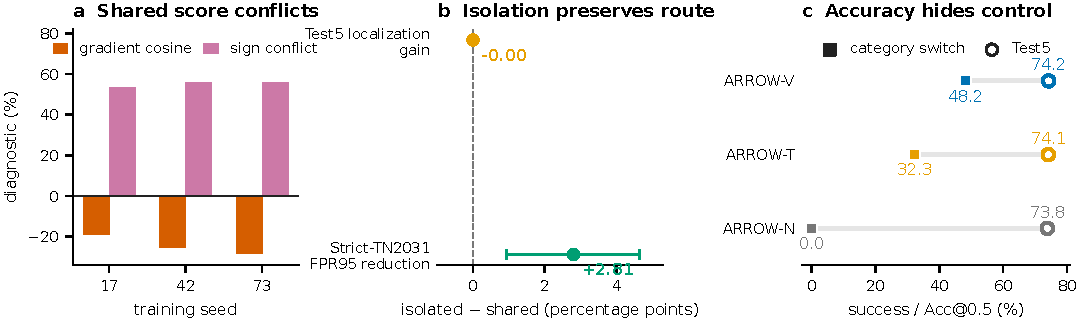
\includegraphics[width=\textwidth]{figures/fig3_mechanism_controllability.pdf}%
  }{\fbox{\parbox[c][1.15in][c]{0.96\textwidth}{\centering
    Gradient conflict, paired ownership effects, and V/T/N category-switch
    controllability generated from registry CSVs.}}}
  \caption{Mechanism evidence.  Shared-duty gradients conflict, structural
  isolation preserves localization while improving rejection, and nearly flat
  standard accuracy hides large differences in category controllability.}
  \label{fig:mechanism}
\end{figure*}

% Generated by paper/scripts/make_main_tables.py.
\begin{table}[t]
\centering
\caption{Admission cues.  FineCops columns use one exact-support matched
surface; the switch panel changes only the named category cue.}
\label{tab:admission}
\scriptsize
\setlength{\tabcolsep}{0.8pt}
\begin{tabular}{lccccc}
\toprule
Cue & Test5$\uparrow$ & Switch$\uparrow$ & P@1$\uparrow$ & Text R@1$\uparrow$ & Image R@1$\uparrow$ \\
\midrule
Visual support & 74.24 $\pm$ 0.09 & 48.24 & 44.16 & 45.05 & 46.14 \\
Category text & 74.12 $\pm$ 0.29 & 32.29 & 43.70 & 44.50 & 45.43 \\
Learned null & 73.83 $\pm$ 0.62 & 0.00 & 42.11 & 42.96 & 43.87 \\
\bottomrule
\end{tabular}
\vspace{2pt}
\parbox{0.98\columnwidth}{\scriptsize Percentages; Test5 is mean $\pm$
sample SD over all three seeds. Visual$-$text switch gain is
+15.95 pp
[$10.81$, $20.83$];
text$-$null is +32.29 pp
[$28.65$, $36.00$]. Visual-support
coverage is 95.60\%; unsupported rows are never counted as rejection.}
\end{table}


\subsection{Endpoint accuracy hides Admission responsibility}
The three capacity-matched cues are close on Test5 but diverge under direct
intervention (Tab.~\ref{tab:admission}, Fig.~\ref{fig:mechanism}).  \arrown
retains 73.83\% Test5 accuracy yet has zero bidirectional category-switch
success.  Canonical text reaches \ArrowTextSwitch\%, and visual support reaches
\ArrowVisualSwitch\%.  The preregistered visual-over-text and text-over-null
confidence intervals both exclude zero.  Matched FineCops results repeat the
ordering on positive P@1 and both negative types.  The supported conclusion is
that visual examples provide category evidence beyond the name, not that
support pixels are required for every correct localization.

% Generated by paper/scripts/make_main_tables.py.
\begin{table}[t]
\centering
\caption{External rejection transfer. FineCops uses standard expression-only
inputs; gRefCOCO is explicitly restricted to single-target/no-target rows.}
\label{tab:external}
\textbf{(a) FineCops-Ref full test}\\[2pt]
\scriptsize
\setlength{\tabcolsep}{1.0pt}
\begin{tabular}{lccccc}
\toprule
Route & P@1$\uparrow$ & T R@1$\uparrow$ & I R@1$\uparrow$ & T AUC$\uparrow$ & I AUC$\uparrow$ \\
\midrule
MM-GDINO-T (published) & 48.45 & 38.69 & 43.14 & 53.98 & 56.52 \\
Original GDINO-T (local) & 44.82 & 41.99 & 41.98 & 54.23 & 53.92 \\
Frozen base & 43.11 & 42.66 & 43.98 & 58.87 & 59.55 \\
Ranking + Abstention & 43.02 & 43.85 & 44.76 & 60.88 & 60.69 \\
\bottomrule
\end{tabular}
\\[5pt]
\textbf{(b) gRefCOCO rejection transfer}\\[2pt]
\scriptsize
\begin{tabular}{llcccc}
\toprule
Slice & Route & AUROC$\uparrow$ & AUPR$\uparrow$ & FPR95$\downarrow$ & Fixed TPR \\
\midrule
Full & Base & 68.95 & 72.01 & 74.10 & -- \\
 & Rejector & 71.75 & 73.81 & 70.83 & 90.10 \\
Rej.-sup.-disj. & Base & 68.69 & 71.92 & 74.97 & -- \\
 & Rejector & 71.50 & 73.73 & 71.16 & 89.72 \\
\bottomrule
\end{tabular}
\\[-1pt]
\parbox{0.98\columnwidth}{\scriptsize T/I denote negative text/image.
The published MM-GDINO-T row is context, not a local or paired comparison.
The local original row loads the unmodified OGC checkpoint with its native
max-token score.  AUC uses the pinned official evaluator's historical
level-1-positive scope for every FineCops row. Fixed TPR uses the sealed source
source threshold; it is never refit. Multi-target gRefCOCO is excluded.}
\end{table}


\subsection{Rejection ordering transfers; the operating point does not}
Table~\ref{tab:external} reports both external surfaces.  On complete
FineCops, the text-cue \arrowt route trails the published
MM-GDINO-T positive P@1 but has numerically higher negative-expression and
negative-image Recall@1.  Because \arrowt receives the structured target noun,
this published row is a reference rather than an input-matched contrast.  We
claim transfer against our same-forward frozen controls, not FineCops SOTA.
\arrowv's support-conditioned result is kept on its matched covered surface and
is never substituted into a full-test row.

On gRefCOCO Full, AUROC rises from 0.6895 to 0.7175 and FPR95 falls from 0.7410
to 0.7083.  On Rejector-supervision-disjoint, AUROC rises from 0.6869 to 0.7150
and FPR95 falls from 0.7497 to 0.7116; all four paired gain intervals exclude
zero.  Because Stage-A saw every image, this controls rejector-supervision
overlap only.  It is evidence about no-target rejection rather than a new
localization domain.

\begin{figure}[t]
  \centering
  \IfFileExists{figures/fig4_external_transfer.pdf}{%
    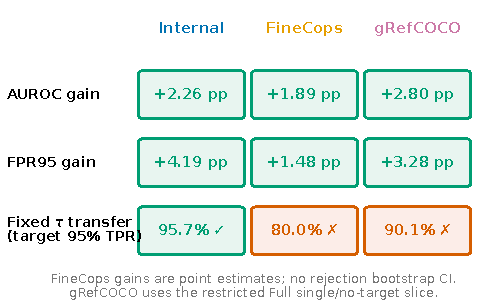
\includegraphics[width=\columnwidth]{figures/fig4_external_transfer.pdf}%
  }{\fbox{\parbox[c][1.05in][c]{0.96\columnwidth}{\centering
    Internal, FineCops, and gRefCOCO rejection ordering versus fixed-threshold
    positive TPR, shown on separate aligned axes.}}}
  \caption{Relative rejection discrimination improves across three negative
  constructions.  The internally sealed threshold reaches its intended source
  operating point but yields only \ArrowFineCopsFixedTPR\% TPR on FineCops and
  \ArrowGrefFixedTPR\% on gRefCOCO.  Thresholds are never fit externally.}
  \label{fig:external}
\end{figure}

Figure~\ref{fig:external} shows that the fixed source threshold under-accepts
external positives.  Improved
AUROC and dataset-normalized FPR95 are compatible with this shift: \method
learns a more transferable positive-versus-negative ordering, while score
offset, scale, and tails remain domain-dependent.  Cross-domain operating-point
calibration is a separate, unresolved problem.

\section{Limitations}
\label{sec:limitations}

\textbf{Single-target scope.} \method emits at most one box or abstention and
does not solve variable-cardinality multi-target GREC.  Our gRefCOCO result is
explicitly a single/no-target slice.

\textbf{Domain-dependent calibration.} FineCops is descriptive and gRefCOCO
paired-confirmed; the sealed threshold misses 95\% TPR on both.  We do not
claim a universal confidence scale.

\textbf{Visual-support coverage.} \arrowv relies on a frozen exact-match
support taxonomy and covers \ArrowFineCopsCoverage\% of FineCops positives.
\arrowt provides a full-coverage text-cue route; covered and full-test
universes are not directly compared.

\textbf{Exposure caveats.} FineCops is annotation/task-zero-shot rather than
fully image-disjoint.  gRefCOCO's Rejector-supervision-disjoint subset excludes
only rejection train/calibration images; all evaluated images were seen during
Stage-A, and many positive expressions overlap the sealed RefCOCO test input.

\textbf{Positive-grounding ceiling and verification scope.} \method targets
selective reliability and does not establish FineCops positive P@1 SOTA.
Strict negatives are proposal-covered SAM3+VLM verified, not image-global or
all-query verified.

\section{Conclusion}
\label{sec:conclusion}

\method factorizes selective grounding into candidate Admission,
complete-expression Ranking, and sample-level Abstention, improving held-out
localization and verified rejection while category interventions expose hidden
responsibility.  Matched owner controls show a conditional mechanism:
isolation protects one conflict-prone representation, whereas broad pretrained
and task-tuned MM-GDINO representations support wide sharing despite negative
tails.  Conflict is diagnostic, not prescriptive: responsibilities can remain
distinct under shared parameters, while rejection ordering transfers better
than a fixed threshold.

\FloatBarrier

\phantomsection\label{paper:references-start}
{\small
\bibliographystyle{ieeenat_fullname}
\bibliography{references}
}
\end{document}
